\section{Задание 4.}

\textbf{Условие.}

Найдите разложение функции $f(x)$ в цепную дробь и ряд Маклорена. Придайте аргументу $x$ из области 
сходимости некоторое значение и сравните точность разложений по нескольким первым членам разложения. 

\[f(x) = \arcsin \frac{x}{2}\]

\vspace{10mm}

\textbf{Решение.}

Найдем ряд Маклорена для $f(x) = \arcsin \frac{x}{2}$. По формуле

\[T_n(x) = f(0) + \frac{f^\prime(0)}{1!} x + \frac{f^{\prime\prime}(0)}{2!} x^2 + \dots + \frac{f^{(n)}(0)}{n!} x^n\]

ряд Маклорена для $\arcsin x$ из первый 5 членов будет таким:

$\displaystyle T_4(x) = f(0) + \frac{f^\prime(0)}{1!} x + \frac{f^{\prime\prime}(0)}{2!} x^2 + \frac{f^{(3)}(0)}{3!} x^3 + \frac{f^{(4)}(0)}{4!} x^4$

Воспользовавшись вычислительной техникой, получаем $f^\prime(x) = \frac{1}{2}, f^{\prime\prime}(0) = 0, f^{(3)}(0) = \frac{1}{8}, f^{(4)}(0) = 0$,
а \fbox{$\displaystyle T_4(x) = \frac{x}{2} + \frac{x^3}{48}$}

\vspace{6mm}

Теперь разложим $f(x)$ в цепную дробь. Найдем разложение для $\arctg x$ в виде дроби $\displaystyle \frac{x}{1 + z}$;
так как $\displaystyle \arctg^\prime x = \frac{1}{1 + x^2}$, $\left(\frac{x}{1 + z}\right) = \frac{1}{1 + x^2}$ или 
$\displaystyle (1 + x^2)xz^\prime + (1 - x^2)z + z^2 = x^2$. 

Пользуясь полученными вычислениями из пособия \enquote{Приложение цепных дробей и из обощений к вопросам приближенного анализа}
\footnote{\enquote{Приложение цепных дробей и их обобщений к вопросам приближенного анализа}, Хованский А.Н., 1956, стр. 114},
получаем $\displaystyle z = \frac{x^2}{3 + \frac{4x^2}{5 + \frac{9x^2}{7 + \dots}}}$

Из этого $\displaystyle \arctg x = \frac{x}{1 + \Phi_1(x)}$, где $\Phi_k(x) = \frac{k^2x^2}{2k + 1 + \Phi_{k + 1}(x)}$

Зная, что $\arcsin x = \arctg \frac{x}{\sqrt{1 - x^2}}$, получаем 
$\displaystyle f(x) = \arcsin \frac{x}{2} = \frac{\frac{x}{2\sqrt{1 - (\frac{x}{2})^2}}}{1 + \frac{\frac{x^2}{4 - x^2}}{3 + \dots}} = 
\frac{\frac{x}{\sqrt{4 - x^2}}}{1 + \Phi_1(x)}$, где $\displaystyle \Phi_k(x) = \frac{\frac{k^2x^2}{4 - x^2}}{2k + 1 + \Phi_{k + 1}(x)}$

Для первых 4 членов $\Phi_k$ получаем \fbox{$\displaystyle R_4(x) = \frac{\frac{x}{\sqrt{4 - x^2}}}{1 + \frac{\frac{x^2}{4 - x^2}}{3 + \frac{\frac{4x^2}{4 - x^2}}{5 + \frac{\frac{9x^2}{4 - x^2}}{7 + \frac{\frac{16x^2}{4 - x^2}}{9}}}}}$}

Пользуясь графическим калькулятором Geogebra, изобразим $f(x), T_4(x)$ и $R_4(x)$ на графике (\url{https://www.geogebra.org/calculator/mr6grjv9}):

\begin{center}
    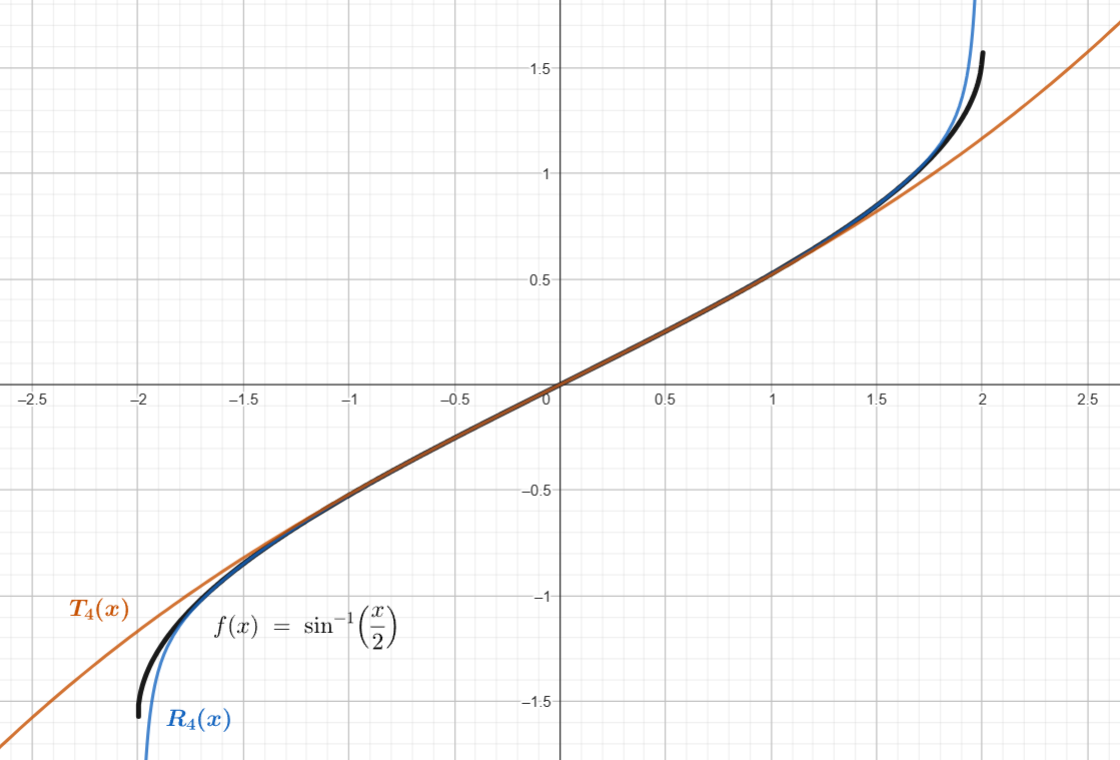
\includegraphics[width=0.8\textwidth]{images/4-01}
\end{center}

Сравним их значения для $x_0 = 1 \in [-2;2]$:

\begin{gather*}
    f(x_0) = 0.5235987755983 \\
    T_4(x_0) = 0.5208333333333 \\
    R_4(x_0) = 0.5236003198863
\end{gather*}

Как можно заметить, для первых 5 членов ряд Маклорена дает ошибку $\frac{|T_4(x_0) - f(x_0)|}{f(x_0)} \cdot 100\% = 0.528\%$, 
разложение в цепную дробь - $\frac{|R_4(x_0) - f(x_0)|}{f(x_0)} \cdot 100\% = 0.000294\%$

\clearpage
